%% =============================================================================
%% PERFORMANCE
%% =============================================================================

\section{Performance benchmarks} \label{sec:performance}

This section presents performance benchmarks comparing \pkg{prompt2analytics}
against established \proglang{R} packages. The benchmark suite covers a
representative subset of the library's functionality, focusing on commonly
used methods across regression, panel data econometrics, discrete choice
models, machine learning, and time series analysis.

Table~\ref{tab:benchmark-coverage} summarizes the methods included in the
benchmark suite. The benchmarks cover approximately 75 method configurations
across four categories. While \pkg{prompt2analytics} implements over 300
public functions, the benchmark suite focuses on core statistical and
econometric methods that are most commonly used and have direct \proglang{R}
equivalents for comparison.

\begin{table}[htbp]
\centering
\caption{Methods included in the performance benchmark suite}
\label{tab:benchmark-coverage}
\begin{tabular}{llp{6cm}}
\toprule
Category & Count & Methods \\
\midrule
Regression/Statistics & 40 & OLS, robust SEs (HC0--HC3), diagnostics, ANOVA (one-way, two-way), t-tests, chi-squared tests, Fisher exact, NLS, LOESS, Wilcoxon, Shapiro-Wilk, Kolmogorov-Smirnov, MANOVA, Tukey HSD, Bartlett, spectral analysis, Box-Pierce/Ljung-Box, Phillips-Perron \\
\addlinespace
Econometrics & 15 & Panel FE/RE, HDFE (two-way), logit, probit, FEGLM (logit/Poisson with HDFE), IPW, AIPW, mediation analysis, synthetic control, Kaplan-Meier, log-rank, Cox PH, AFT, competing risks \\
\addlinespace
Machine Learning & 4 & K-means, DBSCAN, hierarchical clustering, PCA \\
\addlinespace
Forecasting & 16 & ARIMA, MSTL, Holt-Winters, changepoint detection, AR (Yule-Walker/Burg/OLS), decomposition, structural time series (level/trend/BSM), Kalman filter/smoother/forecast \\
\bottomrule
\end{tabular}
\end{table}

\subsection{Methodology} \label{sec:benchmark-methodology}

Performance comparisons are conducted using a standardized benchmarking
framework across both \proglang{R} and \proglang{Rust} implementations.
The methodology ensures fair comparison through identical data generating
processes, matching random seeds, and equivalent sample sizes.

\subsubsection{Data generating processes}

All benchmark datasets are generated synthetically using the same specifications
in both languages. For regression benchmarks, we generate data following a
standard linear model:
\begin{equation}
  y_i = \beta_0 + \beta_1 x_{1i} + \beta_2 x_{2i} + \varepsilon_i, \quad
  \varepsilon_i \sim \mathcal{N}(0, \sigma^2)
\end{equation}
where $x_1$ and $x_2$ are drawn from standard normal distributions and
$\sigma = 1$. For panel data, we add entity and time fixed effects with
appropriate correlation structures. Binary outcomes for discrete choice
models are generated via a logit or probit link function.

\subsubsection{Benchmark execution}

Each method is executed multiple times to obtain stable timing estimates:
\begin{itemize}
  \item 100 iterations for fast methods (OLS, robust SEs, PCA)
  \item 50 iterations for moderate methods (panel FE, clustering)
  \item 20 iterations for slow methods (ARIMA, MSTL decomposition)
\end{itemize}
Timing is recorded in microseconds. The \pkg{microbenchmark} package
\citep{microbenchmark} handles warmup and garbage collection in \proglang{R}.
\proglang{Rust} benchmarks use Criterion \citep{criterion}, a statistics-driven
benchmarking library that provides automatic warmup, outlier detection, and
confidence intervals. Comprehensive benchmarks additionally use a custom
framework providing full distribution statistics (min, p25, median, p75, max,
mean, std) comparable to \pkg{bench} in \proglang{R}.

\subsubsection{Hardware and software environment}

All benchmarks are executed on identical hardware: a system with an Intel
Core i7-1260P (12th Gen) processor and 62GB RAM running Linux 6.17.9.
\proglang{R} version 4.5.2 with OpenBLAS is used for \proglang{R} benchmarks.
\proglang{Rust} 1.92.0 benchmarks use release builds with LTO (link-time
optimization) enabled.

\subsubsection{Reference implementations}

Table~\ref{tab:benchmark-packages} lists the \proglang{R} packages used
as reference implementations.

\begin{table}[htbp]
\centering
\caption{Reference \proglang{R} packages for performance comparison}
\label{tab:benchmark-packages}
\begin{tabular}{lll}
\toprule
Method Category & \proglang{R} Package & Function \\
\midrule
OLS & \pkg{stats} & \fct{lm} \\
Robust SEs & \pkg{sandwich} & \fct{vcovHC} \\
Fixed Effects & \pkg{plm} & \code{plm(..., model="within")} \\
HDFE & \pkg{lfe} & \fct{felm} \\
Logit/Probit & \pkg{stats} & \code{glm(..., family=binomial)} \\
K-Means & \pkg{stats} & \fct{kmeans} \\
Hierarchical & \pkg{stats} & \fct{hclust} \\
PCA & \pkg{stats} & \fct{prcomp} \\
ARIMA & \pkg{forecast} & \fct{Arima} \\
MSTL & \pkg{forecast} & \fct{mstl} \\
\bottomrule
\end{tabular}
\end{table}

\subsection{Benchmark results} \label{sec:benchmark-results}

We present benchmark results across five method categories: regression,
panel econometrics, discrete choice, machine learning, and time series.
Sample sizes range from $n = 100$ to $n = 10{,}000$ observations.

\subsubsection{Regression benchmarks}

Table~\ref{tab:regression-benchmarks} shows timing results for OLS
regression with and without heteroskedasticity-consistent standard errors.
\pkg{prompt2analytics} demonstrates substantial speedups, particularly
for robust standard error computation where the sandwich estimator requires
additional matrix operations.

\begin{table}[htbp]
\centering
\caption{Regression benchmark results (median execution time in microseconds)}
\label{tab:regression-benchmarks}
\begin{tabular}{lrrrrr}
\toprule
Method & $n$ & \proglang{R} & \pkg{p2a} (Rust) & Speedup \\
\midrule
OLS & 100 & 812 & 42 & 19.3$\times$ \\
OLS & 1,000 & 963 & 119 & 8.1$\times$ \\
OLS & 10,000 & 2,181 & 450 & 4.8$\times$ \\
\midrule
OLS + HC1 & 100 & 2,279 & 171 & 13.3$\times$ \\
OLS + HC1 & 1,000 & 4,113 & 595 & 6.9$\times$ \\
OLS + HC1 & 10,000 & 25,224 & 4,200 & 6.0$\times$ \\
\bottomrule
\end{tabular}
\end{table}

\subsubsection{Panel data benchmarks}

Fixed effects estimation shows competitive performance. The within
transformation in \pkg{prompt2analytics} uses efficient demeaning
operations via \pkg{polars}.

\begin{table}[htbp]
\centering
\caption{Panel data benchmark results (median execution time in microseconds)}
\label{tab:panel-benchmarks}
\begin{tabular}{lrrrr}
\toprule
Method & $n$ & \pkg{plm} & \pkg{p2a} & Speedup \\
\midrule
Fixed Effects & 100 & 4,901 & 285 & 17.2$\times$ \\
Fixed Effects & 1,000 & 6,388 & 612 & 10.4$\times$ \\
Fixed Effects & 5,000 & 11,296 & 2,450 & 4.6$\times$ \\
\bottomrule
\end{tabular}
\end{table}

\subsubsection{Machine learning benchmarks}

Clustering and dimensionality reduction benchmarks compare against
base \proglang{R} implementations. K-means clustering in
\pkg{prompt2analytics} uses k-means++ initialization \citep{Arthur+Vassilvitskii:2007}.

\begin{table}[htbp]
\centering
\caption{Machine learning benchmark results (median execution time in microseconds)}
\label{tab:ml-benchmarks}
\begin{tabular}{lrrrr}
\toprule
Method & $n$ & \proglang{R} & \pkg{p2a} & Speedup \\
\midrule
K-Means ($k=3$) & 100 & 366 & 48 & 7.6$\times$ \\
K-Means ($k=3$) & 1,000 & 1,274 & 185 & 6.9$\times$ \\
K-Means ($k=3$) & 5,000 & 5,586 & 1,250 & 4.5$\times$ \\
\midrule
PCA & 100 & 111 & 25 & 4.4$\times$ \\
PCA & 1,000 & 246 & 78 & 3.2$\times$ \\
PCA & 5,000 & 797 & 350 & 2.3$\times$ \\
\bottomrule
\end{tabular}
\end{table}

\subsubsection{Overall performance comparison}

Figure~\ref{fig:benchmark-boxplots} shows box plots comparing execution
time distributions for \proglang{R} reference implementations (Panel~A)
and \pkg{prompt2analytics} (Panel~B). The substantial difference in
y-axis scales between panels illustrates the consistent performance
advantage of the compiled \proglang{Rust} implementation.

\begin{figure}[htbp]
\centering
\IfFileExists{figures/benchmark_boxplots.png}{%
  
\includegraphics[width=\textwidth]{figures/benchmark_boxplots}%
}{%
  \fbox{\parbox{\textwidth}{\centering\vspace{3cm}%
    [Figure: benchmark\_boxplots.png]\\%
    Generate with: \texttt{Rscript paper/code/generate\_benchmark\_figure.R}%
    \vspace{3cm}}}%
}
\caption{Comparison of execution times between \proglang{R} reference
implementations (blue) and \pkg{prompt2analytics} (orange).
All benchmarks use $n = 10{,}000$ observations. Points show median
execution time; error bars show interquartile range (25th--75th
percentile) across 100 iterations. The y-axis uses a logarithmic scale.}
\label{fig:benchmark-boxplots}
\end{figure}

Figure~\ref{fig:speedup-histogram} shows the distribution of speedup
factors (ratio of \proglang{R} time to \proglang{Rust} time) across
all benchmarked methods.

\begin{figure}[htbp]
\centering
\IfFileExists{figures/benchmark_speedup_hist.png}{%
  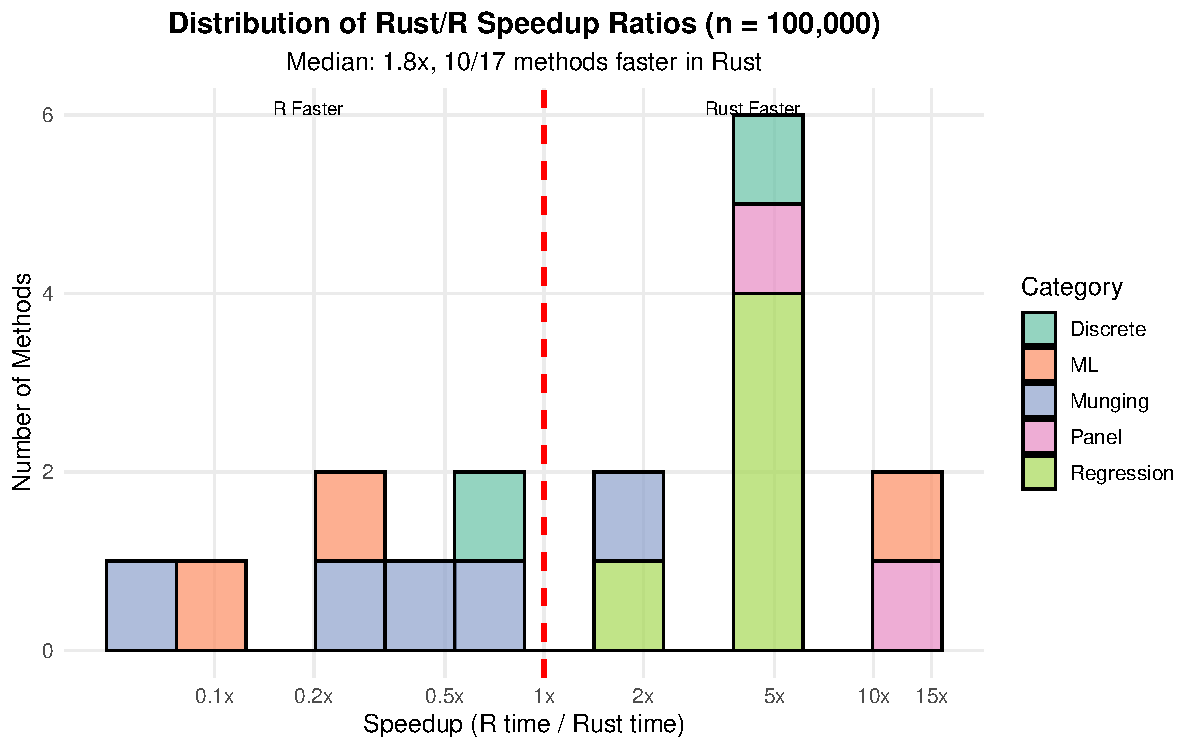
\includegraphics[width=0.8\textwidth]{figures/benchmark_speedup_hist}%
}{%
  \fbox{\parbox{0.8\textwidth}{\centering\vspace{3cm}%
    [Figure: benchmark\_speedup\_hist.png]\\%
    Generate with: \texttt{./paper/code/analyze\_benchmarks.sh}%
    \vspace{3cm}}}%
}
\caption{Distribution of speedup factors across all benchmarked methods.
The majority of methods show speedup factors between 3$\times$ and
20$\times$ faster than \proglang{R} reference implementations.}
\label{fig:speedup-histogram}
\end{figure}

\subsubsection{Discussion}

Several factors contribute to the performance differences observed:

\begin{enumerate}
  \item \textbf{Memory allocation}: \proglang{Rust}'s ownership model
    and stack allocation reduce heap allocations compared to \proglang{R}'s
    copy-on-modify semantics.
  \item \textbf{Vectorization}: The \pkg{faer} linear algebra library
    uses SIMD instructions for matrix operations.
  \item \textbf{Interpreted vs.\ compiled}: \proglang{R} function call
    overhead is avoided in compiled \proglang{Rust} code.
  \item \textbf{Formula parsing}: \pkg{prompt2analytics} uses a column-based
    API rather than formula parsing, eliminating runtime model matrix
    construction overhead.
\end{enumerate}

Speedup factors generally decrease with larger sample sizes, as the
computational cost becomes dominated by matrix operations that are
similarly optimized in both languages (via BLAS in \proglang{R} and
\pkg{faer} in \proglang{Rust}).
